% This must be in the first 5 lines to tell arXiv to use pdfLaTeX, which is strongly recommended.
\pdfoutput=1
% In particular, the hyperref package requires pdfLaTeX in order to break URLs across lines.

\documentclass[11pt]{article}

% Remove the "review" option to generate the final version.
\usepackage[]{acl}
\usepackage{subfig}
% Standard package includes
\usepackage{times}
\usepackage{latexsym}
\usepackage{amsmath}
% For proper rendering and hyphenation of words containing Latin characters (including in bib files)
\usepackage[T1]{fontenc}
% For Vietnamese characters
% \usepackage[T5]{fontenc}
% See https://www.latex-project.org/help/documentation/encguide.pdf for other character sets

% This assumes your files are encoded as UTF8
\usepackage[utf8]{inputenc}

% This is not strictly necessary, and may be commented out,
% but it will improve the layout of the manuscript,
% and will typically save some space.
\usepackage{microtype}
\usepackage{array, boldline, makecell, booktabs}
\usepackage{graphicx} % DO NOT CHANGE THIS
% If the title and author information does not fit in the area allocated, uncomment the following
%
%\setlength\titlebox{<dim>}
%
% and set <dim> to something 5cm or larger.

\title{DISTANT-CTO: A Zero Cost, Distantly Supervised Approach to Improve Low-Resource Entity Extraction Using Clinical Trials Literature}

% Author information can be set in various styles:
% For several authors from the same institution:
 \author{Anjani Dhrangadhariya \and Henning M{\"u}ller\\
         University of Geneva (UNIGE), Geneva, Switzerland \\ University of Applied Sciences Western Switzerland (HES-SO), Sierre, Switzerland \\ \texttt{\{anjani.dhrangadhariya,henning.mueller\}@hevs.ch} }
% if the names do not fit well on one line use
%         Author 1 \\ {\bf Author 2} \\ ... \\ {\bf Author n} \\
% For authors from different institutions:
% \author{Author 1 \\ Address line \\  ... \\ Address line
%         \And  ... \And
%         Author n \\ Address line \\ ... \\ Address line}
% To start a seperate ``row'' of authors use \AND, as in
% \author{Author 1 \\ Address line \\  ... \\ Address line
%         \AND
%         Author 2 \\ Address line \\ ... \\ Address line \And
%         Author 3 \\ Address line \\ ... \\ Address line}

%\author{First Author \\
%  Affiliation / Address line 1 \\
%  Affiliation / Address line 2 \\
%  Affiliation / Address line 3 \\
%  \texttt{email@domain} \\\And
%  Second Author \\
%  Affiliation / Address line 1 \\
%  Affiliation / Address line 2 \\
%  Affiliation / Address line 3 \\
%  \texttt{email@domain} \\}

\begin{document}
\maketitle
\begin{abstract}
PICO recognition is an information extraction task for identifying participant, intervention, comparator, and outcome information from clinical literature.
Manually identifying PICO information is the most time-consuming step for conducting systematic reviews (SR), which is already labor-intensive.
A lack of diversified and large, annotated corpora restricts innovation and adoption of automated PICO recognition systems.
The largest-available PICO entity/span corpus is manually annotated which is too expensive for a majority of the scientific community.
To break through the bottleneck, we propose DISTANT-CTO, a novel distantly supervised PICO entity extraction approach using the clinical trials literature, to generate a massive weakly-labeled dataset with more than a million ``Intervention'' and ``Comparator'' entity annotations.
We train distant NER (named-entity recognition) models using this weakly-labeled dataset and demonstrate that it outperforms even the sophisticated models trained on the manually annotated dataset with a 2\% F1 improvement over the Intervention entity of the PICO benchmark and more than 5\% improvement when combined with the manually annotated dataset.
We investigate the generalizability of our approach and gain an impressive F1 score on another domain-specific PICO benchmark.
The approach is not only zero-cost but is also scalable for a constant stream of PICO entity annotations.
\end{abstract}
%
\section{Introduction}
\label{sec:intro}
%
Primary care physicians rely on systematic reviews (SRs) for informed decision-making.
SRs are conducted to objectively answer clinical questions and require going through a rigorous process of manually screening tens of thousands of clinical studies to identify terms describing PICO.
PICO information identification is crucial to appraise the relevance of a clinical study for answering the clinical question at hand.
A study is only included for writing SRs if it mentions relevant PICO information.
Manual PICO information screening for a single SR consumes more than 12 months of two medical experts' time.
The process can be automated using information extraction (IE) by directly pointing the human reviewers to the correct PICO descriptions.
Automation will accelerate the overall process of writing SRs while reducing the burden on health professionals who are required to manually screen for PICO entities.

Automating PICO entity detection has garnered lower interest than other biomedical NER tasks because of the lack of publicly available entity annotated corpora.
The largest publicly-available PICO entity/span dataset (EBM-PICO) contains only 5000 annotated abstracts, some of which were annotated through crowd-sourcing and others by hired medical experts~\cite{nye2018corpus}.
Crowd-sourcing involves hiring non-expert workers that require intensive training that is not commonly affordable.
Hiring medical experts for annotation is equally often too expensive.
In general, extracting PICO entities/spans is somewhat tricky because of high disagreement between human annotators on the exact spans constituting the mentions.
This leads to human errors in hand-labeled corpora.
Hand-labeled datasets are static and prohibit quick manual re-labeling in case of human errors or when a downstream task requires new entities.
For example, PICO entities extend to PICOS, where S denotes the ``study type'' of included evidence.
%In all the previous studies using EBM-PICO as a benchmark, the ``Intervention'' entity extraction had the worst performance, as this class is composed of several intervention sub-classes leading to a class heterogeneity challenge~\cite{cardellino2017low}.

Distant supervision (DS) is a data-centric approach that allows generating massive weakly annotated datasets without human annotators and has previously been used to create large relation extraction corpora for the general and biomedical domains.
To address the challenges above and democratize PICO entity recognition, we propose DISTANT-CTO, a distantly supervised and scalable approach to obtaining clinical trials annotations.
We take an integrative approach combining methods of semi-supervised learning (SSL) and gestalt pattern matching (GPM) to develop a continuously extensible dataset.
We successfully demonstrate this approach for the ``Intervention'' and ``Comparator'' entity annotations as proof of concept (POC).


We summarize our contributions as follows:
%
\begin{itemize}
    \item We develop a zero-cost, data-centric approach using DS to obtain ``Intervention'' and ``Comparator'' entity annotations.
    \item We develop and make publicly available a large weakly-labeled dataset from more than 300,000 clinical trials. The dataset offers about a million sentences with more than 977,682 annotations across 11 semantic types.
    \item We improve the state-of-the-art by 2\% macro-F1 on the previously most poor-performing ``Intervention'' entity extraction on the EBM-PICO benchmark corpus without using costly manually labeled data and by 5\% when combined with manually labeled data.
\end{itemize}
%
%
%
\section{Related Work}
\label{sec:relworks}
%
A decade of automatic PICO information extraction was limited to sentence-level due to the unavailability of entity-annotated corpora~\citep{boudin2010combining, huang2011classification, huang2013pico, wallace2016extracting, jin2018pico}.
The release of the EBM-PICO corpus paved the way for the community to improve upon the PICO entity/span extraction task.~\citep{nye2018corpus}.
The corpus is biased towards pharma intervention classes overshadowing non-pharma ones leading to a substandard performance on it in the previous SOTA fully-supervised PICO entity/span recognition models~\citep{beltagy2019scibert,brockmeier2019improving,zhang2020unlocking} and weakly supervised model~\citep{liu2021sent2span}.
Small-scale annotation projects cannot capture the range and variation of the PICO descriptions spanning the entirety of clinical trials literature.
At some point, applications of such static corpora will confront the problem of insufficient and irrelevant annotations.
Manual annotation projects are neither affordable nor scalable for every lab, limiting innovation.

A plethora of DS methods have been previously explored for large-scale relation extraction but not for (named) entity extraction~\cite{etzioni2008open,smirnova2018relation,adelani2020distant}.
Entity extraction in high-impact clinical and biomedical domains largely relies on small expert annotated datasets.
Commonly, obtaining weak annotations using DS rely on aligning terms (a word or phrase) from ontologies onto the unstructured text ~\citep{giannakopoulos2017unsupervised,yang2018distantly,peng2019distantly,hedderich2021anea}.
Ontologies are structured, standardized data sources that do not capture various writing variations from clinical literature.
Weak annotations obtained using custom-built rules like regular expressions are restricted by either task or worse even by entity type~\cite{ratner2017snorkel,safranchik2020weakly,fries2021ontology}.
Bootstrapping approaches like label propagation (LP) still require an expert annotated dataset to obtain pseudo annotations for previously unlabeled data samples~\cite{bing2017bootstrapping}.
It is hence not zero-cost.

Our work focuses on overcoming the discussed bottlenecks using a data-centric DS approach to generate a large clinical entity annotated corpus and train a downstream NER model to assess if it yields adequate results.
Unlike the reviewed DS approaches, our approach does not use ontologies or rules or LP but rather uses GPM for flexibly aligning structured text in a clinical trials database to the free-text fields in the same database using an adaptable internal scoring scheme.
%
%
%
\section{Data}
\label{sec:data}
%
ClinicalTrials.gov (CTO hereafter) documents more than 350,000 human clinical studies conducted around the globe.
The trial's principal investigator enters and updates information about each study stored in CTO.
It includes the title and description of the clinical trial, participant's eligibility criteria, participant disease and demographics, interventions evaluated, outcomes, \textit{etc.}
CTO allows programmatic access to this vast amount of information in the JSON (JavaScript Object Notation) format.
The information is stored as a combination of structured tabular and unstructured free-text (see Figure~\ref{fig:CTO_example}).
The `OfficialTitle' and `BriefTitle' tags in the JSON respectively store the official and shorter version of the study title in an unstructured free-text format.
The `BriefSummary' and `DetailedDescription' tags store study summaries.
Interventions used in the study are stored under the `InterventionName' tag and their synonyms under `InterventionOtherName' tag each of which could be linked to their broad semantic type (drug, device, behavioral, procedural, biological, dietary supplement, diagnostic test, radiation, genetic, combination product, other) mentioned under the `InterventionType' tag.
As each intervention name is linked to its semantic type, this becomes a structured information store.
The `InterventionDescription' tag describes intervention administration procedures often in a detailed passage.
%
\begin{figure*}[t]
\centering
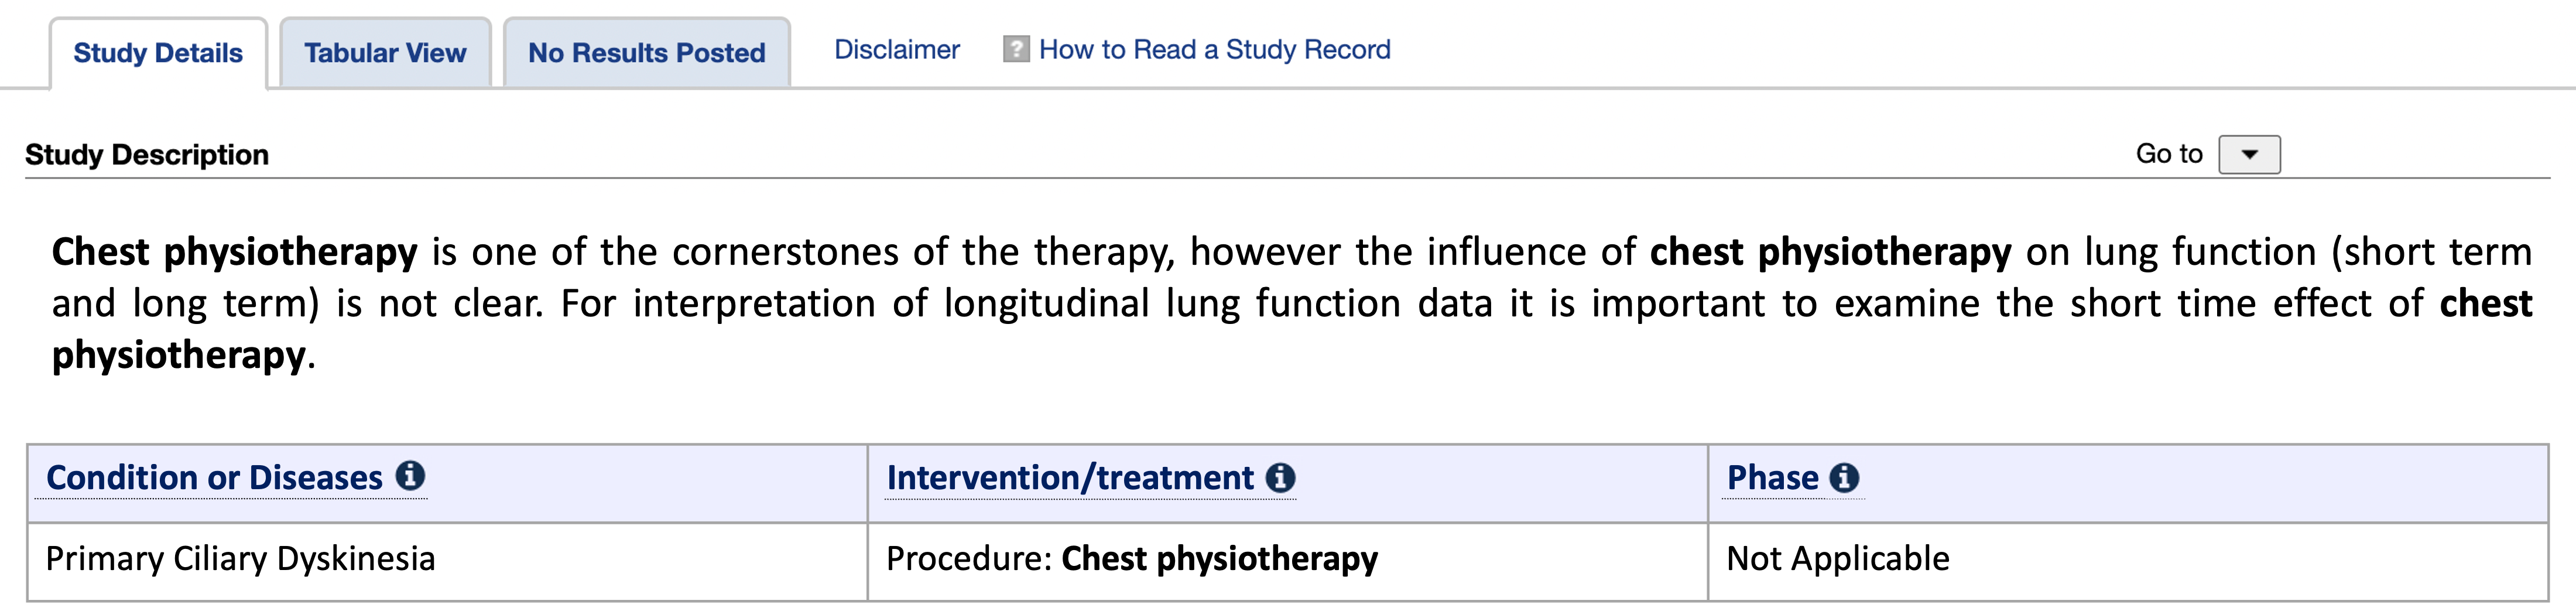
\includegraphics[width=0.98\textwidth]{figures/example_figure1.png}
\caption{An example CTO record (ID - NCT01929356) to demonstrate the information storage format which is a combination of structured table and unstructured text.}
\label{fig:CTO_example}
\end{figure*}
%
%
%
%
\section{Approach}
\label{sec:methods}
%
The approach is schematically illustrated in Figure~\ref{fig:approach} and is described below.
%
\subsection{Distant Supervision}
\label{subsec:ds}
%
Distantly supervised (DS) information extraction (IE) is an efficient SSL method~\cite{etzioni2008open,wen2019efficient}.
It is used when the task at hand has 1) some strongly-labeled data, 2) abundant unlabeled data, and 3) a weak-labeling function that could sample from this unlabeled data and label them using a heuristic function.
This labeling function is a heuristic algorithm that uses a heuristic to label the unlabeled data~\cite{pinto2003table, greaves2014relation}.
It results in a weakly-labeled dataset with potential label noise.
DS-IE models can then collectively use this strongly-labeled and weakly-labeled training data to give the final output.
%
\subsection{Gestalt Pattern Matching}
\label{subsec_gsp}
%
In entity extraction, the most common form of DS is to heuristically align terms from a structured information source onto the unstructured text~\cite{wen2019efficient}.
When flexible, this heuristic boils down to a substring matching problem. The weak-labeling function matches the longest common substring (LCS) between the structured term and unstructured text.
Gestalt Pattern Matching (GPM), also known as Ratcliff/Obershelp similarity algorithm, is a string-matching algorithm for determining the similarity of two strings.
The similarity between two strings $S_{1}$ and $S_{2}$ is measured by the formula, calculating twice the number of matching characters $K_{m}$ divided by the total length $|S_{1}| + |S_{2}|$ of both strings.
Matching characters are identified by the LCS algorithm followed by recursively finding matching characters in the non-matching regions on either side from both strings~\cite{ratcliff1988pattern}.
$Similarity$ ranges between 0, which means no match, and 1, which means a complete match of the two strings.
%
\begin{gather}
  Similarity (S) = \dfrac{ 2 K_{m}}{|S_{1}| + |S_{2}|} \: ; \: 0 \leq	 S \leq	 1
 \end{gather}
%
%
\paragraph{Difflib: }
\label{difflib}
It is a python module providing a {\tt sequencematcher} function that extends the GPM algorithm for comparing pairs of strings.
{\tt sequencematcher} finds the longest contiguous subsequence between the sequence pair without the ``junk'' elements such as blank lines or white spaces.
The same idea is then applied recursively to the flanks of the sequences to the left and the right of the matching subsequence.
This yields matching sequences that appear normal to the human eye.
%
\subsection{Candidate Generation}
\label{subsec:candgen}
%
We define candidate generation as the process of automatically generating entity-annotated sentences.
%
\paragraph{Assumption and Problem formulation: }
As ``Intervention'' and ``Comparator'' entities represent interventions in two different roles in clinical trials and semantically the same classes, they are clubbed into a single ``Intervention'' entity class.
Let each CTO record JSON file be $r_i \in \boldsymbol{R}, i = \{ 1, 2, ... , I \}$.
Let the intervention terms in `InterventionName' tags and `InterventionOtherName' tags be the intervention source $S = \{ s_1, s_2, ... , s_m \}$ used in the study $r_i$.
Each intervention term $s_i \in S$ is linked to intervention class from `InterventionType' tag converting it into a tuple of $ \langle s_{class}, s_{name} \rangle$, $s_{name} =$ intervention term and $s_{class} =$ intervention category.
$s_{name}$ is a sequence of words $\{ y_1, y_2, ... , y_n \}, n = \{ 1, 2, ... , N \} $.
Let each sentence $t_i = \{ x_1, x_2, ... , x_m \}, m = \{ 1, 2, ... , M \}$ in the `BriefSummary', `DetailedDescription', `BriefTitle', `OfficialTitle' and `InterventionDescription' be a part of the intervention target set $T$.
We assume that for each $s_{name}$ in $r_i$ there could exist a mapping to $t_i$ meaning $s_{name}$ is possibly either completely or partially mentioned in the $t_i$ (see Figure~\ref{fig:CTO_example}).
Our goal is to build a scalable and adaptable candidate generation pipeline that maps each $s_{name}$ from the structured intervention source $S$ to the target sentences $t_i \in T$ (if a loose mapping exists).
In this prototypical work, we focus on \textit{almost} direct matches between the $s_{name}$ and $t_i$ and keep the order-free matches for future work.
%
%
\paragraph{Approach}
For each individual CTO record $r_i$, we extract all $s_{name} \in S$ and $t_i \in T$ from the locally stored CTO dump.
Both $S$ and $T$ are preprocessed by lower-casing, replacing hyphens and multiple trailing spaces with a single space and removal of Unicode characters.
Given a $s_{name}$ and $t_i$, our aim is to identify and score (if identified) the mapping between both sequences.
To map and score alignment from the $s_{name}$ to $t_i$, we use a distant supervision labeling function $LF_{ds}$ which is a combination of the {\tt sequencematcher} function and an internal scoring function to fetch almost direct annotations.
The {\tt sequencematcher} function takes as input $s_{name}$ and $t_i$ and outputs several matching blocks $d_{block} \in D_{blocks}$ between both strings.
These matching blocks between the two strings are calculated using a modified gestalt pattern matching algorithm as elaborated in \ref{difflib}.
Each $d_{block} = \langle MatchPos_{t}, MatchPos_{s}, MatchLen \rangle $. 
$MatchPos_{t}$ is the start of the match in $t_i$, $MatchPos_{s}$ is the start of the match in $s_{name}$ and $MatchLen$ is number of characters matching between the both.
{\tt sequencematcher} provides an internal scoring function called as {\tt ratio} that returns a similarity score between the two sequences being matched.
We do not use {\tt ratio} because it returns an overall matching score between the two full sequences $s_{name}$ and $t_i$ rather than a match score for $s_{name}$ and $d_{block}$.
Instead, to identify the matching blocks that correspond to an exact match between an entire $s_{name}$ and a part of $t_i$, we calculate a match score $d_s$ for each matching block output by {\tt sequencematcher} using equation~\ref{eq:internalscore} which is dividing the number of matching characters in the match block $d_{block}$ by number of characters in $s_{name}$.
%
\begin{gather}
\label{eq:internalscore}
  d_s = \dfrac{ MatchLen }{ |s_{name}| } \: ; \: 0 \leq d_s \leq 1
\end{gather}
%
Any $d_{block}$ with the $d_s$ score of 1.0 is considered as complete match and then the $s_{name}$ corresponding to the $d_{block}$ is mapped onto sentence $t_i$ to generate a positive annotation sentence $a_{+} \in A_{+}$.
Using the $d_{block}$ with only the match score 1.0 leads to missing out on several entities leading to an incomplete noisy weakly annotated dataset.
Taking this into consideration, we retrieve the $d_{block}$ matching with $d_s$ score of 0.9 as fairly-accurate partial matches.
We used a validation set to relax the choice of similarity match score $d_s$ to 0.9.
We relax the labeling function $LF_{ds}$ to match bigrams in source terms to the targets.
In the real-world data, not all sentences in clinical trial literature mention the intervention name and therefore in addition to the positive annotation sentences we require negative annotation sentences.
We take $t_i$ and $s_{name}$ where no parts of $d_{block}$ scored $d_s$ more than 0.2 to generate the negative annotation sentences $a_{-} \in A_{-}$.
%For the targets $t$ comprising more than one sentence and containing both $a_{+}$ and $a_{-}$ candidates, we slice them into groups of four.
We call all these sequences comprised of the positive and the negative entity annotated sentences $A_{+-}$ our weakly annotated dataset.
Next, for all $A_{+-}$ instances we fetch part-of-the-speech (POS) tags using {\tt POS-tagger} from NLTK (Natural Language Toolkit) resulting into $A_{+-POS}$.
We call the resulting dataset DISTANT-CTO set.
POS tags are added as additional features as they have shown to help model generalization~\cite{augenstein2017generalisation}.
{\tt difflib} in combination with the internal scoring function are previously unexplored for automatic entity annotation generation.
It has to be noted that the method depends on availability of short source texts with the possibility that they will be mentioned in longer target texts.
%
%
%
\begin{figure*}[ht]
    \centering
    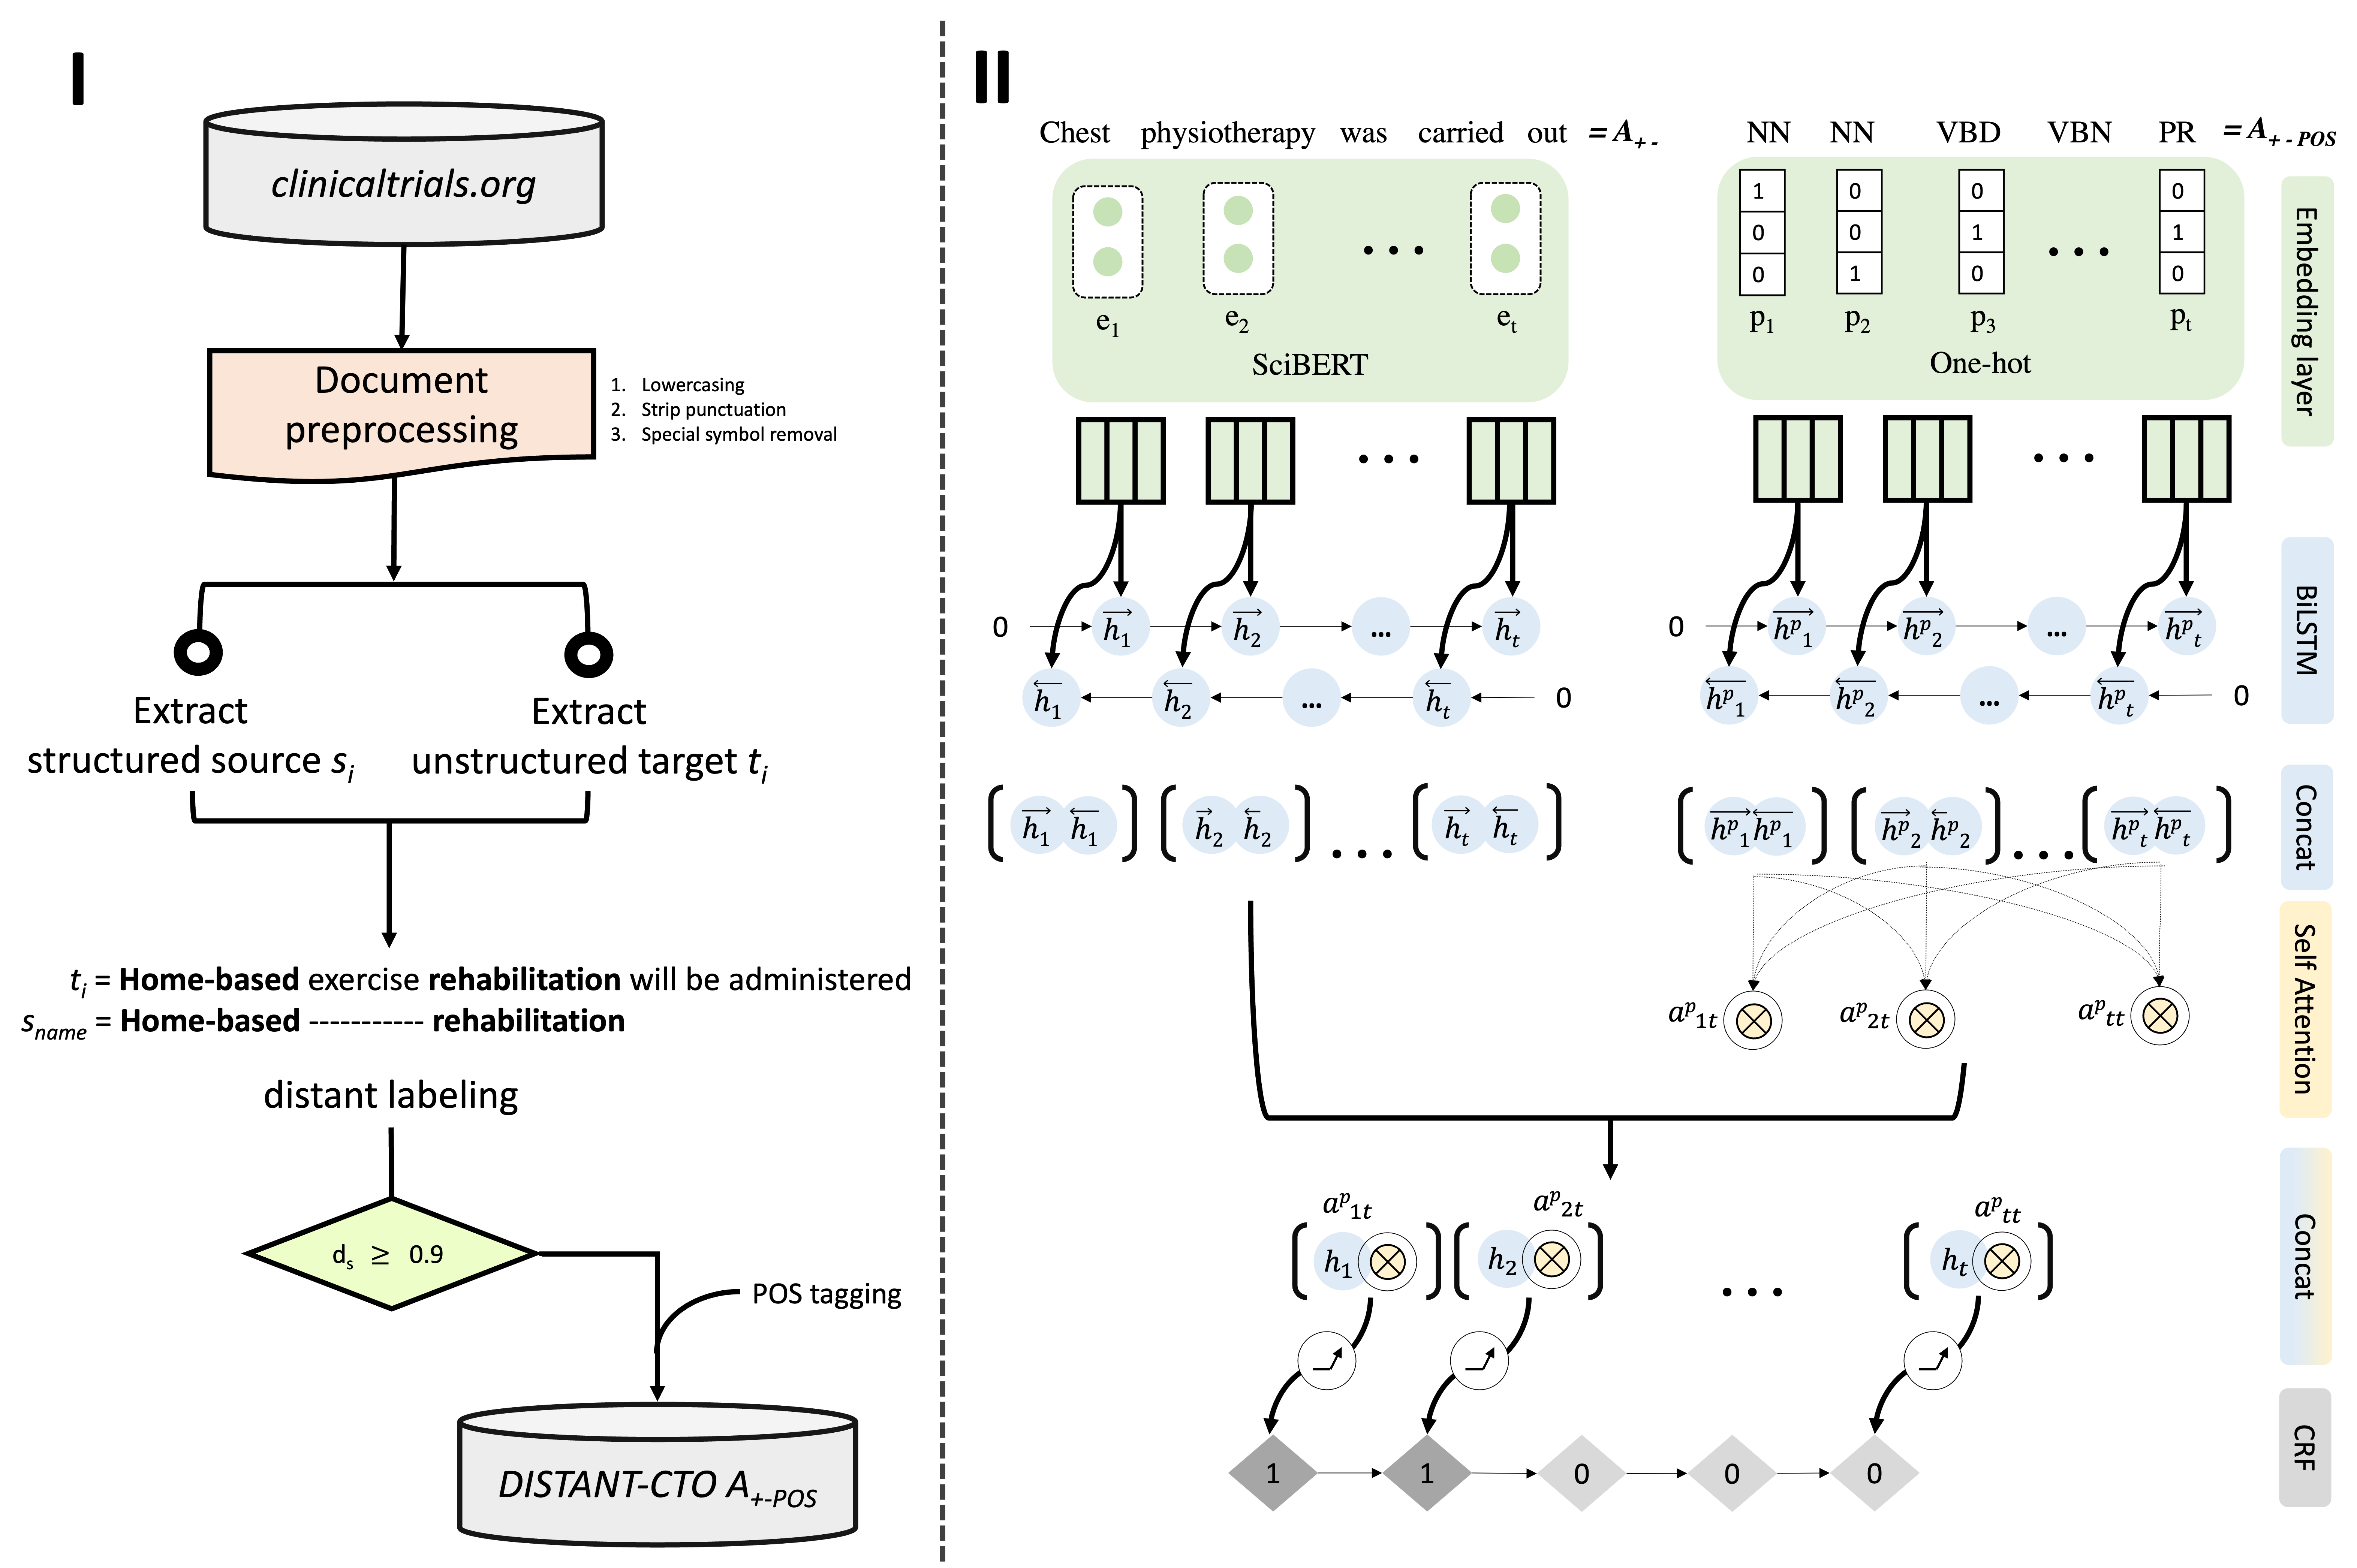
\includegraphics[width=0.98\textwidth]{figures/process.png}
    \caption{DISTANT-CTO approach - I) Distantly-supervised candidate generation approach, and II) Distantly-supervised NER model architecture.}
    \label{fig:approach}
\end{figure*}
%
%
%
\subsection{Model Training}
\label{subsec:training}
%
We train an end-to-end distant NER model on $A_{+-POS}$ using the architecture explained below.
%
\paragraph{1. Feature Extraction:}
%
%Open-domain pre-trained language models (LM) like BERT, ULMFit and GPT rule out the need for heavy feature engineering and also tackle the the challenge of out-of-vocabulary (OOV) words using the WordPiece tokenizer and byte pair encoding (BPE)~\cite{devlin2018bert,joshi2019comparison}.
%Unfortunately, they encode limited semantic and syntactic information for domain-specific tasks.
To capture the domain-specific information, we used SciBERT, which was continually pretrained and domain adapted on the scientific literature from semantic scholar~\cite{gururangan2020don}.
The models used SciBERT to tokenize the text input $A_{+-}$ into encoded tokens $x_{t}$ and extract dense, contextual vectors $e_{t}$ from $x_{t}$ at each time-step $t$~\cite{beltagy2019scibert}.
POS-inputs $A_{+-POS}$ were one-hot encoded into $p_{t}$ vectors.
%
\paragraph{2. Feature transformation:}
%
To further fine-tune to the training corpus, the model stacked a bidirectional LSTM (BiLSTM) on top of the SciBERT~\cite{hochreiter1997long}.
A BiLSTM layer encodes the text into a $(\overrightarrow{h})$ and $(\overleftarrow{h})$  vector using the current token embedding input $e_{t}$ and the previous hidden state $h_{t-1}$ in both the directions.
$\overrightarrow{h}$ and $\overleftarrow{h}$ were shallow concatenated $([\overrightarrow{h}; \overleftarrow{h}])$ into $h_{t}$ and used as the input for the next layer.
Similarly, the one-hot encoded POS-vectors $p_{t}$ underwent feature transformation and were concatenated $([\overrightarrow{h}_{POS}; \overleftarrow{h}_{POS}])$ into POS-features $h^{p}_{t}$.
%
\paragraph{3. Self-attention: }
%
Next, the model stacked a single-head self-attention layer that calculated for each POS-tag feature at time $t$ in the sequence a weighted average of the feature representation of all other POS-tag features in the sequence $a^{p}_{t}$ ~\cite{vaswani2017attention}.
This improves the signal-to-noise ratio by out-weighting important POS features.
%Self-attention weights for each POS-tag were calculated by multiplying hidden representation $h^{p}_{t}$ with randomly initialized Query $q$ and Key $k$ weights, which were further multiplied with each other to obtain attention weighted vectors.
%Finally, the obtained attention weights were multiplied with the Value (V) matrix which was obtained by multiplication between a randomly initialized weight matrix $v$ and $h_{t}$ finally obtaining scaled attention-weighted vectors $a^{p}_{t}$.
Attention-weighted POS features and $h_{t}$ were shallow concatenated into $([a^{p}_{t}; h_{t}])$ vector.
%
\paragraph{4. Decoder:}
%
The attention-weighted representation $([a^{p}_{t}; h_{t}])$ was fed to a linear layer to predict the tag emission sequence $\hat{y_{t}}$ followed by a CRF layer that takes as input the $\hat{y_{t}}$ sequence along with the true tag $y_{t}$ sequence~\cite{huang2015bidirectional}.
%CRF is a graph-based model suitable for learning tag sequence dependencies from the training set and has shown to outperform softmax classifiers.
%
%
%
\section{Experiments}
\label{sec:experiments}
%
The experiments were designed to evaluate the performance of the distant NER models trained with the DISTANT-CTO set alone \textit{vs.} DISTANT-CTO set in combination with the EBM-PICO training set.
The EBM-PICO training set is naturally composed of both positive and negative annotation sentences, but for the DISTANT-CTO, we artificially generated the negative sentences $A_{-}$.
To evaluate the impact of these negative annotation sentences, we perform ablation experiments, training the models only with positive annotation sentences $A_{+}$.
Finally, we also evaluate the performance when training using the entity annotations with match score $d_s = 1.0$ alone \textit{vs.} entity annotations with $d_s \geq 0.9$.
A simple SciBERT-CRF model trained using positive annotation sentences $A_{+}$ was used as the baseline. 
Transformer-based models incorporate sequence order and self-attention components, so our baseline served to check the impact of removing costly BiLSTM and self-attention modules.
%
%
\subsection{Benchmark datasets}
\label{subsec:benchmark}
%
We evaluate our weakly annotated dataset and the NER model on the following PICO benchmarks.
%
\begin{enumerate}
    \item \textbf{EBM-PICO gold.} The EBM-PICO dataset developed by Nye \textit{et al.} consists of 5000 PICO entity/span annotated documents~\footnote{A single document consists of a title and an abstract.}. It comes pre-divided into a training set (n=4,933) annotated through crowd-sourcing and an expert annotated test set (n=191) for evaluation purposes. We use the training set for combined training experiments and the test set for evaluation.
    \item \textbf{Physio set.} A test set comprising 153 PICO entity/span annotated documents from Physiotherapy and Rehabilitation RCTs (Randomized Controlled Trials) was used as an additional benchmark to evaluate the generalization power of our approach for this sub-domain~\cite{dhrangadhariya2021end}.
\end{enumerate}
%
%
%
\subsection{Experimental Setup}
\label{subsec:expsetup}
%
We define the following experimental setups based on the motivations described in section~\ref{sec:experiments}:
\begin{itemize}
\item \textbf{Exp 1.0 distant $A_{+-}$ c[1,0.9] wPOS} The setup is composed of SciBERT BiLSTM CRF trained on the surface form (text) and attention-weighted POS inputs using DISTANT-CTO set comprising entity-annotated sentences $A_{+-}$ with $d_s \geq 0.9$.
    \item \textbf{Exp 1.1 distant $A_{+-}$ c[1] wPOS} The setup is composed of SciBERT BiLSTM CRF trained on the surface form and attention-weighted POS inputs using the DISTANT-CTO set comprising only the entity-annotated sentences $A_{+-}$ with $d_s = 1.0$.
    \item \textbf{Exp 1.2 distant $A_{+}$ c[1] wPOS} The setup is composed of SciBERT BiLSTM CRF trained on the surface forms and attention-weighted POS inputs using DISTANT-CTO set comprising only the $d_s =$ 1.0 annotations. The negative annotation sentences were removed in this case and the system was trained with positive annotated candidates $A_{+}$ only.
    \item \textbf{Exp 1.3 distant $A_{+}$ c[1] POS $\neg$ BiLSTM attention } The setup is composed of SciBERT CRF trained on the surface form inputs using DISTANT-CTO set comprising only the $d_s =$ 1.0 annotations with only positive annotated candidates $A_{+}$. Attention weights were removed from the POS inputs. This setup was used as the baseline.
    \item \textbf{Exp 2.0 - Exp 2.3 } These experiments are identical to their series 1.x counterparts except that the models are trained on a combination of the DISTANT-CTO with the EBM-PICO training set. Exp 2.3 using SciBERT-CRF architecture was used as another baseline.
\end{itemize}
%
%
%
\subsection{Evaluation}
\label{subsec:eval}
%
%\paragraph{Candidate generation }
To evaluate the quality of automatic annotation using the DISTANT-CTO approach, we performed manual annotation of the ``Intervention'' class over 200 randomly selected samples from the dataset and compared it to the automatic annotations.

%\paragraph{Model training }
Model evaluation was carried out by predicting the ``Intervention'' tokens for both benchmarks.
Each experiment was conducted thrice with three random seeds (0, 1, and 42), and the average metrics (Precision, Recall, and F1) over three repetitions were reported.
We evaluated the statistical significance of our best model using the paired student's t-test as described in~\cite{dror2018hitchhiker}.
Further experimental details are in the Appendix.
%
%
%
\section{Results}
\label{sec:results}
%
This section reports empirical results for the candidate generation process, evaluation for the annotation quality of DISTANT-CTO approach using the validation sets (see Table~\ref{tab:cangen_eval}), and the average of the performance metrics and standard deviation $\sigma$ over three random seeds on both benchmark datasets for the described NER experiments (see Table~\ref{tab:results_modeltraining}).
We compare the performance of our weakly-supervised NER models with the previous SOTA fully supervised (FS) methods that train on the EBM-PICO training set and evaluate on EBM-PICO gold and also a weakly supervised approach  (see Table~\ref{tab:modeltrain_comp}).
These models were separately trained for each of the PICO entities/spans and also clubbed the ``Intervention'' and ``Comparator'' together.
%Therefore, the comparison is valid.
%Sentence-level PICO recognition methods are not comparable to that of entity-level.
%
%
%
\subsection{Candidate Generation}
\label{subsec:res_cand}
%
A total of 360,395 CTO records were downloaded as of March 2021.
From all the downloaded CTO records, we extract 200,545 unique (391,286 redundant) intervention names from the aforementioned intervention sources.
Out of the 391,286 intervention terms retrieved, 104,433 terms were successfully mapped to one of the target sentences with the $d_s =$ 1.0, and 3084 more were mapped with a score of 0.9.
Adding $d_s \geq$ 0.9 mappings did not increase the total number of annotated sentences, but it did increase the number of annotations obtained in each sentence.
Table~\ref{table:res_candgen} shows the total number of intervention annotations obtained from mapping the source terms to target sentences.
%
\begin{table}[!htbp]
\centering
\begin{tabular}{lr|r}
\Xhline{1pt} \textbf{Annotation level} & \textbf{$d_s = 1.0$} & \textbf{$ 1.0 < d_s \geq 0.9$} \\ \Xhline{1pt}
mention-level & 943,284 & 17,199 \\
token-level & 1,515,868 & 43,096 \\
\Xhline{1pt}
\end{tabular}
\caption{Token-level and mention-level intervention annotations obtained in the weakly annotated DISTANT-CTO dataset grouped by their $d_s$ scores.}
\label{table:res_candgen} 
\end{table}
%
%
%
%Metrics for the manual evaluation of DISTANT-CTO using the validation set show that adding annotations with $d_s$ of 0.9 increases the recall by 3\% and hence the overall F1, however, leading to an expected drop in the precision (see Table ~\ref{tab:cangen_eval}).
Metrics for the manual evaluation of DISTANT-CTO using the validation set show that adding annotations with $d_s \geq$ 0.9 increases the recall by 3\%, but lead to an expected drop in the precision (see Table ~\ref{tab:cangen_eval}).
%Finer characteristics of the DISTANT-CTO set are explained in the Appendix.

\begin{table}[!htbp]
\centering
\begin{tabular}{lrrr}
\hline \textbf{Match score} & \textbf{P} & \textbf{R} & \textbf{F1} \\ \hline
$d_s = 1.0$ & 0.86 & 0.80 & 0.83 \\
$d_s \geq 0.9$ & 0.84 & 0.83 & 0.84 \\
\hline
\end{tabular}
\caption{Macro-averaged evaluation metrics for the $d_s =$ 1.0 and $\protect\geq 0.9$ entity annotations for the validation set detailed in the section ~\ref{subsec:eval}}
\label{tab:cangen_eval} 
\end{table}
%
%
%
\subsection{Model Training}
\label{subsec:res_mod}
%
Using the DISTANT-CTO set alone with the NER approach (Exp 1.1 Table~\ref{tab:modeltrain_comp} and \ref{tab:results_modeltraining}) crosses the previous SOTA F1 on the EBM-PICO benchmark by 2\%.
The best overall F1 for both benchmarks is reached upon training the NER models with combined weakly-labeled DISTANT-CTO with the strongly-labeled EBM-PICO dataset (Exp 2.0 Table~\ref{tab:results_modeltraining}) crossing the previous SOTA F1 by 5\% on the EBM-PICO benchmark.
The improvement in F1 for the combined experiments (see Exp 2.1 and 2.0 Table~\ref{tab:results_modeltraining})) is significant when compared to the their best DISTANT-CTO counterparts (see Exp 1.1 Table~\ref{tab:results_modeltraining})).
Using DISTANT-CTO alone has good precision across the experiment series 1.x, but combining it with the EBM-PICO further improves the recall and balances out the F1 in the experiment series 2.x.
Adding the artificially generated $A_{-}$ sentences increases the previous F1 by 5.71\% and 3.77\% (compare Exp 2.2 with Exp 2.1) for both the benchmarks.
Note that adding these negative sentences results in an important improvement of about 9\% in the F1 for the Physio dataset that is specific for the domain of physiotherapy and rehabilitation.
For the combined experiment, the addition of the $d_s \geq$ 0.9 annotations improves the F1 as well by a small margin for the EBM-PICO benchmark (Exp 2.0 I.) but has a marginal performance loss for the Physio benchmark (Exp 2.0 II.).
While using the DISTANT-CTO alone with the $d_s \geq$ 0.9 annotations boosts the precision but downgrades recall thereby reducing the F1 for both benchmarks.
%It is clear from the results that using SciBERT-CRF alone does not yield adequate performance.
%
%
\setlength{\tabcolsep}{4pt} 
\renewcommand{\arraystretch}{1.0}
\begin{table}[hbt!]
    \centering
    \begin{tabular}{llccc}
        \Xhline{1pt}
        % Method & \multicolumn{3}{c}{macro-averaged scores} \\
        Type & Method & P & R & F1 \\
        \Xhline{1pt}
        FS & Nye ~\shortcite{nye2018corpus} &  \textbf{84.00} & 61.00 & 70.00 \\
        FS & Beltagy ~\shortcite{beltagy2019scibert}  & 61.00 & 70.00 & 65.00 \\
        FS & Brockmeier~\shortcite{brockmeier2019improving}  & 69.00 & 47.00 & 56.00 \\
        FS & Stylianou~\shortcite{stylianou2021transformed}  & 69.04 & 79.24 & 73.29 \\
        WS & Liu~\shortcite{liu2021sent2span} & 22.00 & 54.00 & 31.00 \\
        WS & distant-cto (our)  & 83.36 & 70.38 & 75.02 \\
        HS & combined (our) & 76.93  & \textbf{80.17}  & \textbf{78.44} \\
        \Xhline{1pt}
    \end{tabular}
    \caption{Comparison of DISTANT-CTO NER models against the previous SOTA NER methods for ``Intervention'' recognition in terms of macro-averaged precision (P), recall (R), and F1 scores. Boldface represents the best score. Note: FS = Fully Supervised, WS = Weakly Supervised, HS = Hybrid Supervision.}
    \label{tab:modeltrain_comp}
\end{table}
%
%
%
\setlength{\tabcolsep}{4pt} % Default valueapproach: 6pt
\renewcommand{\arraystretch}{1.0}
\begin{table*}[hbt!]
    \centering
    \begin{tabular}{llccc|ccc}
        \Xhline{1pt}
        %Experimental setup & \multicolumn{6}{c}{macro-averaged scores} \\
        %\Xhline{1pt}
        Dataset & Experimental setup & P & R & F1 $\pm\sigma$ & P & R & F1 $\pm\sigma$\\
        \hline 
        & & \multicolumn{3}{c}{I. EBM-PICO gold} & \multicolumn{3}{c}{II. Physio set}  \\
        distant & $A_{+-}$ c[1,0.9] wPOS & 88.85 & 65.39 & 71.27 $\pm$0.007 & 86.13 & 63.70 & 69.14 $\pm$0.003\\
        distant & $A_{+-}$ c[1] wPOS  & 83.36 & 70.38 & \textbf{75.02} $\pm$0.013 & 79.45 & 66.28 & \textbf{70.63} $\pm$0.008\\
        distant & $A_{+}$ c[1] wPOS & 74.85 & 68.74 & 71.25 $\pm$0.005 & 70.52 & 66.37 & 68.14 $\pm$0.002 \\
        distant & $A_{+}$ c[1] POS ¬ BiLSTM att & 85.82 & 64.84 & 70.31 $\pm$0.002 & 79.97 & 60.79 & 65.14 $\pm$0.005 \\
        combined & $A_{+-}$ c[1,0.9] wPOS & 76.93  & 80.17  & \textbf{78.44}* $\pm$0.006 & 75.55  & 79.42 & 77.32 $\pm$0.010\\
        combined & $A_{+-}$ c[1] wPOS & 77.10 & 78.83 & 77.89 $\pm$0.007 & 76.29 & 80.18 & \textbf{78.07}* $\pm$0.009\\
        combined & $A_{+}$ c[1] wPOS & 67.65 & 85.02 & 72.18 $\pm$0.009  & 64.80 & 83.69 & 68.75 $\pm$0.011 \\
        combined & $A_{+}$ c[1] POS ¬ BiLSTM att & 70.91 & 77.38 & 73.60 $\pm$0.025 & 71.50 & 78.40 & 74.38 $\pm$0.020 \\
        \Xhline{1pt}
    \end{tabular}
    \caption{Macro-averaged performance metrics for the NER models trained on weakly annotated DISTANT-CTO alone \textit{vs.} in combination to the strongly annotated EBM-PICO on the two described benchmarks (EBM-PICO gold and the Physio corpus). ``att'' = attention. Bold is the best experiment score. Asterisk (*) denotes a significant F1-score of the experiment to its counterpart in the series 1.x. Significance tested using the paired student's t-test.}
    \label{tab:results_modeltraining}
\end{table*}
%
%
%
%\section{Discussion}
%\label{sec:discussion}
%
%
%
\section{Error Analysis}
\label{subsec:err}
%
\begin{figure}[!tbp]
  \centering
  \subfloat[$d_s = 1.0$]{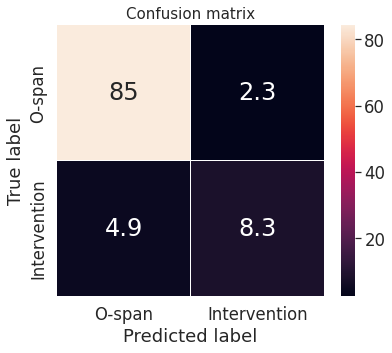
\includegraphics[width=0.48\columnwidth]{figures/conf1_maneval.png}\label{fig:eval1}}
  \hfill
  \subfloat[$d_s \geq 0.9$]{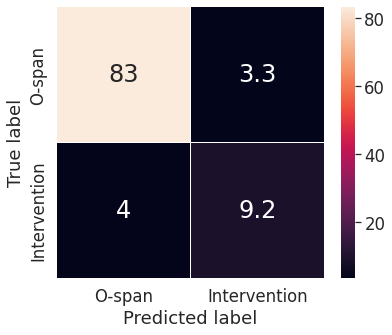
\includegraphics[width=0.48\columnwidth]{figures/conf09_maneval.png}\label{fig:eval2}}
  \caption{Confusion matrices for the evaluation of DISTANT-CTO validation set annotations with a) $d_s = 1.0$ and b) $d_s \geq 0.9$.}
\end{figure}
%
%
%
\subsection{Candidate Generation }
\label{subsec:cand_gen}
%
Confusion matrices (see Figures~\ref{fig:eval1} and ~\ref{fig:eval2}) for manual evaluation of DISTANT-CTO validation set show that relaxing $d_{s}$ from 1.0 to 0.9 does improve the true positives (TP) and reduce false negatives (FN) by 0.9\% for the ``Intervention'' class but also reduce the precision by increasing false positives by 1\%.
Improved recall for the ``Intervention'' class is undoubtedly preferred, and hence it is vital to inspect the cause of false negatives.
A considerable chunk of false negatives was either i) missed intervention abbreviations and the synonyms not mentioned under the sources, or ii) when only the partial intervention name was mentioned in the source, or iii) if specific intervention terms from the source were mentioned in the target but with different word order (see Table~\ref{tab:error_candgen}).
This detailed post-hoc error analysis also revealed that 67\% false negatives fell under non-drug type composite intervention mentions (phrase mentions of more than two words).
For instance, although the term \textit{`Home-based Rehabilitation using Interactive devices'} is expressed in the sentence \textit{`This study investigates clinical outcomes after the rehabilitation by interactive home-based devices.'}, it will remain unmapped to it because the term does not map to the target text using our alignment heuristic.
The problem lies in the lack of naming conventions for non-pharma treatment mentions that are neither clearly identified nor standardized as semantic units\cite{dhrangadhariya2021end}.
There are two possible programmatic solutions to this.
The first is using additional external ontologies as sources of distant supervision which improves coverage of our labeling function to detect further writing variations within the text.
Another solution to matching such source and target text is using order-free string matching algorithms~\cite{apostolico1992combinatorial}.
Using external ontologies solves the issues of missed synonyms, and adding an external dictionary of treatment abbreviations could solve the problem of missed abbreviations~\cite{fries2021ontology}.
We noticed that the ``Comparator'' terms (e.g., placebo, sham, saline, etc.) were often not mentioned as structured sources.
The development of a general comparator term dictionary could improve this.
Improving the coverage and reducing the false negatives (thereby improving recall) using these methodologies suggests an area where future work would be valuable.
Most false positives were a result of bigram matching. 
We will modify fuzzy bigram matching to relevant bigram matching, thereby reducing the occurrences of spurious false-positive bigrams as matches.
Only frequently occurring bigrams from the source will be matched to the targets.
We plan to explore the quality of DISTANT-CTO for $d_s \leq$ 0.9.
%
\begin{table}[ht]
    \centering
    \begin{tabular}{l|r}
    \Xhline{1pt}
       Category & FN count  \\
    \Xhline{1pt}
       Missed synonym  & 168 \\
       Missed abbreviation & 77 \\
       Partial match (incl. boundary errors) & 361 \\
       Missed comparator term & 43 \\
       Reorder & 39 \\
       Total & 688 \\
    \Xhline{1pt}
    \end{tabular}
    \caption{Distribution of the false negatives in the DISTANT-CTO evaluation corpus.}
    \label{tab:error_candgen}
\end{table}
%
%
%
\subsection{Model Training}
\label{subsec:error_modeltrain}
%
%As demonstrated through the results, concatenation of the negative annotation candidates to the positive candidates improves the F1 (compare Exp 1.1 and 2.1 with Exp 1.2 and 2.2) for both benchmarks.
%This shows that the distant NER model requires exploiting the sequence structure and dependencies from both positive and negative examples as in the real-world clinical literature where not all sentences might express the ``Intervention'' entity.
%Addition of $d_s =$ 0.9 annotations while training with DISTANT-CTO alone, deteriorates metrics across the benchmarks increasing the errors (compare Figure~\ref{fig:NEReval1} with~\ref{fig:NEReval2}).
%Addition of $d_s =$ 0.9 annotations, however, improves recall for the combined training with DISTANT-CTO and EBM-PICO for the pharma-dominant dataset.
Manual error analysis was carried out for both the PICO benchmarks, and the error counts for EBM-PICO gold are reported in Table~\ref{tab:error_ner}.
Each token level error was divided into either of the four classes: 1) false negative (FN) - if the entire entity that the token as part of was missed out by the NER model prediction, 2) false positive (FP) - if the entire entity that the token was part of was falsely recognized as ``Intervention'', 3) boundary error (BE) - if the boundary tokens were missed out but otherwise the entity was identified by the NER model prediction, and 4) overlapping error (OE) - if the NER model made an error in the non-peripheral tokens of an otherwise identified entity mention.
Non-peripheral tokens are all the tokens except the first and the last token of the multi-token entity/span.


Models trained on DISTANT-CTO alone had a fewer boundary and overlapping errors, meaning they missed out on many ``Intervention'' entity signals leading to high precision but compromised recall.
On the contrary, NER models trained on combined datasets made twice the more BE and six times more OE.
While most BE and OE in the 1.x series were false negatives, they were false positives in the 2.x series leading to a higher recall.
This could be because the EBM-PICO training set annotated the longest possible intervention span resulting in spans rather than pure entities in the DISTANT-CTO approach.
Combined training set models also picked out names of treatments, surgeries, and enzymes not used as treatments in the RCT as intervention mentions.
A huge chunk of overall FN (including the FN tokens in BE and OE) was for entities with composite intervention terms containing two or more tokens.
We noticed that the NER system also missed several short intervention names and abbreviations.
Overlapping errors occurred when multiple intervention names were mentioned together, separated by either comma or punctuation, or other conjunctions.
The error analysis revealed some issues within EBM-PICO ground truth, which had inconsistencies with the intervention boundaries for whether intervention frequency, dose, and the way of administration should be marked as ``Intervention''.
Several times, the ground truth marked articles preceding the entity and prepositions and punctuation succeeding the entity.
%Appendix has the extended error analysis.
Extended error analysis can be found in the Appendix.
\begin{table}[ht]
\centering
    \begin{tabular}{l|rrrr}
        \Xhline{1pt}
        Exp     & FP & FN & BE & OE\\
         & \multicolumn{4}{c}{EBM-PICO gold} \\
        \Xhline{1pt}
        Exp 1.0 &  819  &  1688  &  559  &  66 \\
        Exp 2.0 &  759  &  1112  &  1278  &  515 \\
        Exp 1.1 &  790  &  1152  &  650  &  55 \\
        Exp 2.1 &  793  &  1039  &  1327 & 517 \\
        \Xhline{1pt}
    \end{tabular}
    \caption{Distribution of the token-level errors made by the corresponding NER models on EBM-PICO gold.}
    \label{tab:error_ner}
\end{table}

%\begin{table}[]
%\centering
%    \begin{tabular}{l|rrrrrr}
%        \Xhline{1pt}
%        Exp     & FP & FN & BE & OE & TP & TN \\
%         & \multicolumn{6}{c}{EBM-PICO gold} \\
%        \Xhline{1pt}
%        Exp 1.0 &  819  &  1688  &  559  &  66 & 1259  & 44515 \\
%        Exp 2.0 &  759  &  1112  &  1278  &  515 & 2100 & 43148 \\
%        Exp 1.1 &  790  &  1152  &  650  &  55 & 1281 & 44584 \\
%        Exp 2.1 &  793  &  1039  &  1327 & 517 & 2100 & 43141 \\
%        \Xhline{1pt}
%    \end{tabular}
%    \caption{Distribution of the token-level errors made by the corresponding NER models on EBM-PICO gold.}
%    \label{tab:error_ner}
%\end{table}
%
%
%
\section{Conclusions and Future Work}
\label{sec:conclusion}
%
We exploit the freely-available clinicaltrials.org (CTO) and distant supervision for developing the largest available weakly annotated database of Intervention-Comparator entities across 11 sub-types.
Using these weak annotations combined with the manual annotations, we train an ``Intervention'' NER model that surpasses current approaches by more than 5\% in terms of F1 on the EBM-PICO gold benchmark and demonstrate strong generalizability on a domain-specific physiotherapy benchmark.
When the same NER model was trained with the weakly annotated dataset alone, it surpassed other approaches by 2\%.
This is a prototypical work, and an automatically obtained dataset with I and C annotations are being extended for the Participant (P), Outcome (O), and Study type (S) entities.
%In the future, we aim to modify the internal matching and scoring to further alleviate the challenge of false negatives that are more prevalent in the composite and long-tail health NEs.
The code and data are available on Github.
%
%
% Entries for the entire Anthology, followed by custom entries
\bibliography{anthology,custom}
\bibliographystyle{acl_natbib}


\appendix

\section{Appendix}
\label{sec:appendix}
%
\subsection{DISTANT-CTO characteristics}
\label{app:char}
%
The total number of entity-level ``Intervention'' mentions in DISTANT-CTO are almost 30 times more than in the EBM-PICO dataset as shown in Table~\ref{table:candcomp}.
For the EBM-PICO training set, 57.48\% of mentions fell under the ``drug'' class and the rest under the six remaining classes.
%
\begin{table}[!htbp]
\centering
\begin{tabular}{lrr}
\Xhline{1pt} \textbf{Total} & \textbf{DISTANT-CTO} & \textbf{EBM-PICO} \\ \Xhline{1pt}
mention-level & 977,682 & 32,890\\
token-level & 1,558,964 & 125,920 \\
\Xhline{1pt}
\end{tabular}
\caption{Comparing the number of ``Intervention'' annotations in DISTANT-CTO \textit{vs.} EBM-PICO.}
\label{table:candcomp} 
\end{table}

Out of all the mention-level annotations in the DISTANT-CTO dataset, 59.90\% corresponded to ``drug'' class and 40\% to the rest of 10 classes.
The pie chart (upper pie in Figure~\ref{app:classdist}) shows the class distribution of the semantic classes for the retrieved ``Intervention'' mentions $s_{name}$ about half of which fall under the ``drug'' (or Pharma) class and the rest under the remaining 10 non-pharma classes.
Out of the total retrieved mentions, almost two-thirds that get mapped to a target $t$ sentences also fall under the ``drug'' class (lower pie in Figure~\ref{app:classdist}).
%
\begin{figure}[ht]
\centering

\includegraphics[width=0.80\columnwidth]{figures/mapped_unmapped_cmyk.jpeg}
\caption{upper) Class distribution for the retrieved ``Intervention'' mentions, and lower) Class distribution for the mapped ``Intervention'' mention.}.
\label{app:classdist}
\end{figure}
%
%
%
Table~\ref{table:int_type10} and~\ref{table:int_type09} shows the number of retrieved intervention mentions by their semantic class \textit{vs.} the percentage of these intervention mentions that get mapped to some target sentence with the match score $d_s$ of 1.0 and score 0.9 respectively.
Notice that collectively the intervention mentions that fall under the non-pharma classes outnumber the pharma (``drug'') mentions.
%
\begin{table}[!htbp]
\centering
\begin{tabular}{lr}
\Xhline{1pt} \textbf{Domain} & \textbf{ retrieved - (mapped)  } \\ \Xhline{1pt}
drug & 184835 (35.50\%) \\
device & 43134 (20.09\%) \\
other & 51703 (16.19\%) \\
procedure & 31630 (21.38\%) \\
behavioral & 33590 (16.03\%) \\
biological & 21225 (22.86\%) \\
dietary supplement & 11699 (25.46\%) \\
radiation & 4134 (20.44\%) \\
diagnostic test & 6742 (10.13\%) \\
combination product & 1070 (14.39\%) \\
genetic & 1524 (07.94\%) \\
all non-pharma & 206,451 (18.80\%)\\
\Xhline{1pt}
\end{tabular}
\caption{Number of intervention mentions retrieved \textit{vs.} percentage mapped with $d_s =$ 1.0}
\label{table:int_type10} 
\end{table}
%
\begin{table}[!htbp]
\centering
\begin{tabular}{lr}
\Xhline{1pt} \textbf{Domain} & \textbf{ retrieved - mapped } \\ \Xhline{1pt}
drug & 184835 (36.22\%) \\
device & 43134 (21.13\%) \\
other & 51703 (16.84\%) \\
procedure & 31630 (22.16\%) \\
behavioral & 33590 (16.44\%) \\
biological & 21225 (24.07\%) \\
dietary supplement & 11699 (27.44\%) \\
radiation & 4134 (21.17\%) \\
diagnostic test & 6742 (10.78\%) \\
combination product & 1070 (14.95\%) \\
genetic & 1524 (08.53\%) \\
all non-pharma & 206,451 (19.64\%)\\
\Xhline{1pt}
\end{tabular}
\caption{Number of intervention mentions retrieved \textit{vs.} percentage mapped with a $d_s$ of 0.9}
\label{table:int_type09} 
\end{table}
%
%
%

Top semantic classes for the most mapped and most unmapped intervention mentions from the total retrieved mentions are shown in the figure~\ref{app:unmapped_class_dist} and~\ref{app:mapped_class_dist}.
As evident from the tables~\ref{table:int_type10} and~\ref{table:int_type09} ``drug'' class intervention mentions are the most mapped followed by ``dietary supplement'' and ``procedure'' classes which also reflects in the pie chart of most mapped lengths and common phrase lengths for each class (see Figure~\ref{app:mapped_class_dist}).
The most frequent phrase length for these classes is one (unigram) and the second most frequent length is two (bigram).
%
\begin{figure}[hbt!]
\centering

\includegraphics[width=1.0\columnwidth]{figures/mapped_class_dist_cmyk.jpeg}
\caption{Top five semantic classes, source intervention mentions from which get mapped to the target.}.
\label{app:mapped_class_dist}
\end{figure}
%
\begin{table}[!htbp]
\centering
\begin{tabular}{lrl}
\Xhline{1pt} \textbf{Domain} & \textbf{ Most common length } \\ \Xhline{1pt}
drug & 1 \\
dietary supplement & 1 \\
biological & 1 \\
procedure & 2 \\
device & 1 \\
\Xhline{1pt}
\end{tabular}
\caption{Lengths for the most mapped classes}
\label{table:len_mapped_classes} 
\end{table}
%
%
The least mapped intervention mention classes are ``combination product'', ``diagnostic test'' and ``behavioral'' (refer figures~\ref{app:unmapped_class_dist}) with most intervention mentions in these classes containing either trigrams or bigrams.
This very well reflects with the numbers in figures~\ref{app:length_mappedunmapped} which shows that trigram and bigram intervention mentions constitute almost half the right pie showing the top phrase lengths for intervention mentions that remain unmapped.
%
\begin{figure}[hbt!]
\centering

\includegraphics[width=1.0\columnwidth]{figures/unmapped_class_dist_cmyk.jpeg}
\caption{Top five semantic classes of the source intervention mentions that remain unmapped to the target.}.
\label{app:unmapped_class_dist}
\end{figure}
%
\begin{table}[!htbp]
\centering
\begin{tabular}{lrl}
\Xhline{1pt} \textbf{Domain} & \textbf{ Most common length } \\ \Xhline{1pt}
device & 3 \\
other & 2 \\
behavioral & 3 \\
diagnostic test & 2 \\
combination product & 3 \\
\Xhline{1pt}
\end{tabular}
\caption{Lengths for the most unmapped classes}
\label{table:len_unmapped_classes} 
\end{table}
%
%
%
\begin{figure*}[hbt!]
\centering

\includegraphics[width=0.80\textwidth]{figures/mention_lengths_distribution_cmyk.jpeg}
\caption{Left) Phrase length distribution of mapped intervention mentions, Right) Phrase length distribution of unmapped intervention mentions.}.
\label{app:length_mappedunmapped}
\end{figure*}
%
%
%
One of the ways to retain some of the missed bigram and trigram intervention mentions is to explore the matches with lower match scores.
The Table~\ref{table:conf9exp} shows some of the $d_s \geq$ 0.9 source-target matches not captured by the $d_s =$ 1.0 constraint because of the difference of either a single missing space or singular-plural differences.
It is also interesting to note that the radiographic procedure ``cystourethrography'' matches the name of the test ``cystourethrogram''.
%
\begin{table*}
\begin{center}
    \begin{tabular}{p{6cm}p{4cm}p{4cm}p{1cm}}
    \Xhline{1pt} \textbf{Characteristic} & \textbf{Source} & \textbf{Target} & \textbf{$d_s$} \\ \Xhline{1pt}
    Single missing space & ``l carnitine'' & ``lcarnitine'' & 0.923\\
    Missing negations & ``no pumice prophylaxis''&  ``pumice prophylaxis''  & 0.900\\
    Plurals & ``punch skin biopsies'' &  ``punch skin biopsy''  & 0.941\\
    Abbreviations & ``rfsh alone'' & ``recombinant fsh alone'' & 0.926\\
    Specific treatment name to generic treatment name & ``biphasic insulin aspart 50'' & ``biphasic insulin aspart'' & 0.923\\
    Procedure matches the instrument & ``cystourethrography'' & ``cystourethrogram'' & 0.900\\
%    Procedure matches the instrument & ``electrocardiography'' & ``electrocardiogram'' & 0.900\\
%    Procedure matches the instrument & ``angiography'' & ``angiogram'' & 0.900\\
    \Xhline{1pt}
    \end{tabular}
\end{center}
\caption{Example ``Intervention'' mentions from CTO that get mapped to target sentences $t$ with a $d_{s}$ of 0.9}
\label{table:conf9exp} 
\end{table*} 
%
%
%
\subsection{Experimental Details}
\label{app:expdet}
%
For the candidate generation process, we did not define any junk elements for using the {\tt sequencematcher} function.
All the NER experiments in this article were conducted in PyTorch and the models were trained for 10 epochs with a mini-batch size of 10 for training and 6 for evaluation.
The maximum sequence length was set to 100 because the average length of each input text sequence was about 68 words.
For both experiments types, either using the DISTANT-CTO alone or with the EBM-PICO training set, 80\% of the data was used for training and 20\% for development.
The [CLS] embeddings from the SciBERT layer were used as features of the input text.
SciBERT was fine-tuned by not freezing weights during the experiments.
The hidden size for LSTM/BiLSTM was set to 512/1024 for the text input embeddings and 20/40 for the POS one-hot embeddings.
ReLU was used as the activation function before feeding emission outputs to the CRF layer.
Model training was optimized using AdamW using a learning rate of 5e-5.
The gradients were clipped to 1.0 to mitigate the problem of exploding gradients.
Due to very specific RAM and GPU requirements for each experiment and the institute's capacity for sharing the GPUs amongst the group members, experiments were carried out on the following GPUs.
Each experiment was carried out on a single GPU without any data and model parallelization.
%
%
\begin{table}[htp]
\centering
\begin{tabular}{l|l|l}
\Xhline{1pt}
\textbf{GPU} & \textbf{RAM} & \textbf{ Experiment }  \\
\Xhline{1pt}
Tesla V100-PCIE-16GB & 1TB  & 1.1, 2.1, 1.3\\
TeslaK80 GPU & 126GB & 1.2, 2.2\\
Tesla V100-PCIE-32GB & 1TB   & 2.0, 1.0, 2.3\\
\Xhline{1pt}
\end{tabular}
\caption{Experiments and the details of GPUs they were carried out on.}
\label{table:exp_gpu} 
\end{table}
%
%
%
\section{Extended Error Analysis}
\label{error_extended}
%
Manual error analysis results for Physio corpus are reported in the Table~\ref{tab:error_hilf_ner}.
FP error count was always lower than the FN error count in the EBM-PICO gold but for the Physio set, the combined NER experiments (series 2.x) lead to a higher FP compared the FN.
The ratio of BE in Exp series 2.x is on an average 1.2 times that of series 1.x.
However, a large chunk of BE in series 1.x are false negatives in contrast to the BE in series 2.x which are false positives.
Upon closer inspection of false-negative BE in series 1.x, we found that they were either missed intervention synonyms inside brackets, missed information accompanying intervention terms like dose, type, medium of intervention, administrator of intervention, or location of administration.
This is due to the fact that distantly supervised annotation does not take into account labeling the additional intervention information except the name.
The addition of the manually annotated EBM-PICO in the combined training experiments reduces the number of false-negative BE.
This is due to the fact that EBM-PICO guidelines required the annotators to mark the longest possible phrase describing intervention including the additional information like dose, mode, medium, and location of administration.


For both the evaluation corpora, the combined NER experiments lead to more TP for the ``Intervention'' class which is vital to PICO entity/span recognition.
This could be the case because the combination of weakly and strongly annotations reduce the percentage of unseen surface forms (words) from both test sets.
27.70\% of the intervention entity surface forms in the EBM-PICO gold benchmark remain unseen in the EBM-PICO training set while for the DISTANT-CTO training set it drops to 21.38\%.
27.29\% of the intervention entity surface forms in the Physio benchmark remain unseen in the EBM-PICO training set while for the DISTANT-CTO training set it drops to 22.97\%.
Combining both training sets leads to a reduction in unseen surface forms to 16.29\% and 15.13\% for the EBM-PICO gold and Physio benchmarks respectively.
\cite{augenstein2017generalisation} has shown that recall on unseen surface forms is significantly lower than on seen surface forms for NER tasks.


\begin{table}[ht]
\centering
    \begin{tabular}{l|rrrr}
        \Xhline{1pt}
        \textbf{Exp}     & \textbf{FP} & \textbf{FN} & \textbf{BE} & \textbf{OE} \\
         & \multicolumn{4}{c}{Physio set} \\
        \Xhline{1pt}
        Exp 1.0 &  963  &  1586  &  654  & 20 \\
        Exp 2.0 & 1168 & 897 & 867  &  347 \\
        Exp 1.1 & 990 & 1420 & 723  & 19  \\
        Exp 2.1 & 1116 & 904 & 1025 & 228 \\
        \Xhline{1pt}
    \end{tabular}
    \caption{Distribution of the token-level errors made by the corresponding NER models on Physio set.}
    \label{tab:error_hilf_ner}
\end{table}

%\begin{table}[]
%\centering
%    \begin{tabular}{l|rrrrrr}
%        \Xhline{1pt}
%        \textbf{Exp}     & \textbf{FP} & \textbf{FN} & \textbf{BE} & \textbf{OE} & \textbf{TP} & \textbf{TN} \\
%         & \multicolumn{6}{c}{Physio set} \\
%        \Xhline{1pt}
%        Exp 1.0 &  963  &  1586  &  654  & 20 & 1123 & 45669 \\
%        Exp 2.0 & 1168 & 897 & 867  &  347 & 2147 & 44591 \\
%        Exp 1.1 & 990 & 1420 & 723  & 19  & 1125 & 45644 \\
%        Exp 2.1 & 1116 & 904 & 1025 & 228 & 2161 & 44523 \\
%        \Xhline{1pt}
%    \end{tabular}
%    \caption{Distribution of the false negatives in the DISTANT-CTO evaluation corpus.}
%    \label{tab:error_hilf_ner}
%\end{table}
%
%
%
\section{Ethical Statement}
\label{ethics}
%
This paper studies clinical NER with a small strongly labeled and a large weakly labeled dataset.
Our investigation neither introduces any social or ethical bias to the model nor amplifies any bias in the data.
We do not foresee any direct social consequences or ethical issues.
%
%
%
\section{License Information}
\label{license}
%
DISTANT-CTO uses all of clinicaltrials.gov (CTO) data that allows downloading and using it given that any publication/distribution states and describes any modifications made to the content of the data.
It is public data that anyone can download and reproduce the outcomes with the code made available on Github.
%
\end{document}